\scanpage{259}
\[
\begin{aligned}
(\unsure{\varphi|\rho}_\infty\tau_\infty P)_{i}
 &\simeq\operatorname{Hom}^i(S,\varphi_\infty\tau_\infty P)\\
 &\simeq\operatorname{Hom}(S[-i],\varphi_\infty\tau_\infty P)\\
 &\simeq\operatorname{Hom}(\tau_\infty S[-i],\tau_\infty P)\\
 &\simeq\underset{\substack{\longrightarrow\\M'\subset S[-i]\\\text{t.q. }S[\unsure{i|-i}]/M'\ \text{négl.}}}{\lim}
 \deleted{\unsure{f|\operatorname{Hom}}}\operatorname{Hom}(M',P)\\
 &\simeq\underset{\substack{\unsure{\rightarrow|-}\\M'\subset S\\\text{t.q. } S/M'\ \text{négl.}}}{\lim}\operatorname{Hom}^i(M',P)\\
 &\simeq\underset{\substack{\longrightarrow\\N}}{\lim}
 \underbrace{\operatorname{Hom}^i(\tau_N S,P)}_{\substack{\rotatebox{90}{$\simeq$}\\\operatorname{Hom}^i(\tau_N S,\tau_{N+i}P)}}\\
 &\simeq\underset{\substack{\unsure{-|\rightarrow}\\N}}{\lim}\operatorname{Hom}(\tau_N(S[-i]),\tau_N P).
\end{aligned}
\]

\figure{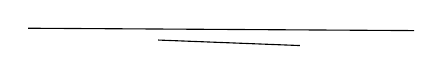
\begin{tikzpicture}[x=1cm,y=1cm]\draw (0,0)--(4.9,-.03) (1.65,-.15)--(3.45,-.22);\end{tikzpicture}}
\diagram{\begin{tikzcd}[ampersand replacement=\&]
\tau_N S\arrow[r,"d^\circ\,0"]\arrow[d,"{\cdot T^{(\ell)}}"']\&P\\
\tau_{N+\ell}(S)\arrow[ur,"{d^\circ\,\deleted{\unsure{0}} \unsure{(\ell)|-\ell|\ell}}"]\&
\end{tikzcd}}
\[
\unsure{\xi|\zeta|\sum}T^{(i)}\overset{T^{(\ell)}}{\longmapsto}\xi c_{i,\ell}T^{(i+\ell)}
\]

\figure{\begin{tikzpicture}[scale=.4]\draw (1,3.7)--(3.6,0) (3.5,-.1)--(0,-3.1)--(-.03,-4);\end{tikzpicture}}
\[
\begin{gathered}
P\in\operatorname{Im\,ess}\varphi_\infty\\
\Updownarrow\\
P\xrightarrow{\sim}\varphi_\infty\tau_\infty P\\
\Updownarrow\\
\operatorname{Hom}^i(S,P)\xrightarrow{\sim}\underset{\substack{\longrightarrow\\N}}{\lim}\operatorname{Hom}^i(\tau_N S,P)
\end{gathered}
\]
a) \uline{injectivité} : $P$ n'a pas d'élément négligeable non nul

b) surjectivité : tout homom. \inserted{homog} d'un \deleted{\unsure{degré}} $\tau_N S$ ds $P$ se prolonge à $S$, ou encore :

toute ext. de $[S/\tau_N S][-i]$ par $P$ est triviale \ldots
% archive sheet number: 258
